\documentclass{article}

\usepackage{arxiv}

\usepackage[utf8]{inputenc}
\usepackage[T1]{fontenc}
\usepackage{hyperref}
\usepackage{url}
\usepackage{booktabs}
\usepackage{amsfonts}
\usepackage{amsmath}
\usepackage{amssymb}
\usepackage{nicefrac}
\usepackage[babel=true]{microtype}
\usepackage{cleveref}
\usepackage{graphicx}
\usepackage{natbib}
\usepackage{doi}
\usepackage{multirow}
\usepackage{array}
\usepackage{algorithm}
\usepackage{algorithmic}

\title{PhyCL-Net: Physics-Inspired Contrastive Lightweight Network for Wearable Fall Detection}

\newif\ifuniqueAffiliation
\uniqueAffiliationtrue

\ifuniqueAffiliation
\author{
	Bowen Zuo\textsuperscript{1}, Siqi Wang\textsuperscript{1}, Junhui Xie\textsuperscript{1}, Sihan Liu\textsuperscript{1}, Xiaojuan Luo\textsuperscript{1,*}\\
	\textsuperscript{1}East China University of Science and Technology, Shanghai 200237, China\\
	\textsuperscript{*}Corresponding author: \texttt{luoxj@ecust.edu.cn}
}
\fi

\renewcommand{\shorttitle}{PhyCL-Net: Lightweight Fall Detection}

\hypersetup{
pdftitle={PhyCL-Net: Physics-Inspired Contrastive Lightweight Network for Wearable Fall Detection},
pdfsubject={cs.LG, cs.CV},
pdfauthor={Bowen Zuo, Siqi Wang, Junhui Xie, Sihan Liu, Xiaojuan Luo},
pdfkeywords={fall detection, wearable sensors, lightweight deep learning, dynamic kernels, attention, contrastive learning, edge inference},
}

\begin{document}
\maketitle

\begin{abstract}
Deploying robust fall detection on resource-constrained wearables presents an accuracy--efficiency dilemma. We propose \textbf{PhyCL-Net}, a time-domain lightweight network that removes the computationally expensive Multi-Scale Spectral Pyramid Analysis (MSPA) while retaining two physics-aware modules: \textit{Physics-Guided Dynamic Kernel (PDK)} for adaptive temporal receptive fields, and \textit{Fall-Aware Attention (FAA)} to emphasize transient impact cues (Jerk). A training-only contrastive objective enhances class separability at zero inference cost. Evaluated on SisFall (12 young adult subjects, ages 19--30) using leave-one-subject-out cross-validation with \textbf{five random seeds}, PhyCL-Net achieves \textbf{98.20\% $\pm$ 0.05\% accuracy} (mean $\pm$ cross-seed std) and \textbf{98.15\% macro-F1}. \textbf{Trade-off:} Removing MSPA reduces TPR@FPR=1\% from 96.02\% to \textbf{93.29\%} but yields \textbf{36.7\%} fewer parameters (1.66M $\to$ 1.05M), \textbf{71.2\%} fewer FLOPs (0.52G $\to$ 0.15G), and \textbf{31.5\%} lower CPU latency (184ms $\to$ 126ms). At the practical operating point (TPR=95\%), PhyCL-Net achieves the lowest false alarm rate (FPR=0.72\%). \textbf{Limitations:} Results are from young adults performing simulated falls; validation on elderly populations (the target demographic) is required before clinical deployment. \textbf{Code:} \url{https://github.com/AlexZander-666/PhyCL_Net}
\end{abstract}

\keywords{fall detection \and wearable sensors \and lightweight deep learning \and contrastive learning \and edge inference}

\section{Introduction}

Falls are a leading cause of injury-related morbidity and mortality among older adults worldwide, creating an urgent need for automated detection systems~\cite{Bergen2016Falls,Newaz2023Methods}. Wearable inertial sensors (accelerometers and gyroscopes) have emerged as the most practical safety layer for continuous monitoring due to their low cost, privacy-preserving nature, and ubiquity in smart devices~\cite{Igual2013Challenges,Chaccour2017Sensors,Casilari2015Wearable}. With the rapid expansion of the Internet of Health Things (IoHT), the paradigm is shifting from cloud-centric processing to \textit{Edge AI}—processing data directly on the wearable node to ensure low latency and offline reliability~\cite{Ramachandran2020Survey,Guo2016Practical}.

However, deploying robust deep learning models on battery-powered edge devices presents a severe \textbf{Accuracy--Efficiency Dilemma}. Recent State-of-the-Art (SOTA) approaches primarily focus on increasing model capacity, utilizing heavy Transformers~\cite{Zerveas2021TST}, complex ensemble methods~\cite{Hussain2023Enhanced}, or explicit time--frequency representations (e.g., Spectrograms, Wavelets)~\cite{wang2019deep,mubashir2013survey}. While these methods achieve high accuracy, they often incur high computational costs (FLOPs) and memory footprints that exceed the constraints of typical Cortex-M microcontrollers used in wearables~\cite{Banbury2021TinyML}.

This work challenges the prevailing assumption that complex frequency-domain analysis is necessary for fall detection. Recent works like ModernTCN~\cite{luo2024moderntcn} have demonstrated that modernized convolutional structures can outperform Transformers in time-series tasks while remaining computationally efficient. From a \textbf{physical kinematics} perspective, routine Activities of Daily Living (ADLs) like walking or jogging are characterized by quasi-periodic low-frequency signals. In contrast, a fall's defining characteristic is the rapid change in acceleration (Jerk magnitude exceeding threshold), which manifests as a high-frequency transient during the 200--800\,ms impact phase~\cite{Bourke2007Threshold,Kangas2008Comparison}. To distinguish falls from high-intensity ADLs (e.g., jumping), we leverage Jerk as the discriminative cue. Transforming such a short, singular transient into the frequency domain (via STFT or spectral pyramids) can diffuse sharp temporal features and introduce unnecessary computational overhead. We hypothesize that a streamlined time-domain encoder, if designed to dynamically adapt to these impulse transients, can achieve SOTA accuracy without the burden of spectral processing.

Guided by this hypothesis, we propose \textbf{PhyCL-Net} (Physics-Inspired Contrastive Lightweight Network). Our baseline architecture, \textbf{MSPA-FAA-PDK}, combines three core modules: Multi-Scale Spectral Pyramid Analysis (MSPA), Fall-Aware Attention (FAA), and Physics-Guided Dynamic Kernel (PDK). PhyCL-Net is derived from MSPA-FAA-PDK by strategically removing the computationally expensive MSPA module while retaining the physics-aware FAA and PDK components. This design choice reflects a pragmatic engineering trade-off: we sacrifice a minor amount of sensitivity at strict low-false-alarm thresholds (TPR@FPR=1\% drops from 96.02\% to 93.29\%) in exchange for substantial efficiency gains (31.5\% latency reduction, 36.7\% parameter reduction) that are critical for real-time wearable deployment.

PhyCL-Net relies on two lightweight, physics-aware mechanisms:

\begin{enumerate}
\item \textbf{Physics-Guided Dynamic Kernel (PDK) Selection:} A module that mimics the eye's accommodation reflex. It dynamically routes information through small kernels (to capture high-frequency impact transients) or large kernels (to capture low-frequency posture transitions) based on the signal's complexity.
\item \textbf{Fall-Aware Attention (FAA):} A mechanism explicitly designed to highlight "Jerk" (rapid derivative changes) and suppress high-energy but sustained ADLs (e.g., running).
\end{enumerate}

To compensate for the reduced parameter count, we introduce a \textbf{training-only} Hierarchical Dual-View Contrastive Learning (HDVCL) framework, building upon recent advances in time-series contrastive learning~\cite{Eldele2021TSTCC,Zhang2022TFC,Zheng2023SimTS}. This "Free Lunch" strategy forces the model to learn more discriminative embeddings during training, allowing us to strip away the auxiliary projection heads during inference, ensuring zero extra deployment cost.

\textbf{Contributions:}
\begin{itemize}
\item \textbf{Pragmatic Accuracy-Efficiency Trade-off:} We demonstrate that removing the spectral branch (MSPA) from the full MSPA-FAA-PDK architecture reduces parameters by \textbf{36.7\%} (1.05M vs. 1.66M), FLOPs by \textbf{71.2\%} (0.15G vs. 0.52G), and CPU latency by \textbf{31.5\%} (126ms vs. 184ms). We transparently report the cost: TPR@FPR=1\% drops from 96.02\% to 93.29\%, a sensitivity reduction at strict thresholds. At the practical operating point (TPR=95\%), PhyCL-Net achieves the lowest FPR (0.72\%) among all tested models.
\item \textbf{Physics-Inspired Architecture:} We propose the PDK and FAA modules, which functionally substitute spectral analysis by explicitly modeling the impulse and derivative characteristics of falls in the time domain. PhyCL-Net retains these physics-aware components while eliminating the computationally expensive MSPA.
\item \textbf{Deployment-Oriented Optimization:} We utilize a contrastive regularization strategy that enhances class separability during training without adding inference parameters. The resulting model maintains robust false alarm control (FPR $<$ 0.72\% at 95\% TPR).
\item \textbf{Rigorous Validation:} On the SisFall dataset (12-subject subset), PhyCL-Net achieves \textbf{98.20\% $\pm$ 0.05\%} accuracy (mean $\pm$ cross-seed std) and \textbf{98.15\%} Macro-F1 under a strict Leave-One-Subject-Out (LOSO) protocol with five independent random seeds, validated with t-distribution confidence intervals.
\end{itemize}


\section{Methodology}

\subsection{Problem Formulation}

Let $\mathcal{D} = \{(\mathbf{X}_i, y_i)\}_{i=1}^N$ be the dataset, where $\mathbf{X}_i \in \mathbb{R}^{C \times L}$ represents a sliding window of inertial sensor data with $C$ channels (e.g., $C=3$ for tri-axial accelerometer) and length $L$. The label $y_i \in \{0, 1\}$ denotes ADL or Fall. Our goal is to learn a lightweight mapping $f_\theta: \mathbb{R}^{C \times L} \to [0,1]$ that maximizes sensitivity to impact transients while minimizing computational operations (FLOPs) and parameters $\theta$.

\subsection{PhyCL-Net Architecture Overview}

To resolve the accuracy--efficiency dilemma, PhyCL-Net abandons the traditional computationally expensive spectral transformation (MSPA). Instead, it adopts a dual-branch time-domain topology:
\begin{itemize}
\item \textbf{Branch A: Physics-Guided Dynamic Kernel (PDK):} Adapts the temporal receptive field size to match the signal's rate of change (Impulse vs. Stationary).
\item \textbf{Branch B: Fall-Aware Attention (FAA):} Focuses on high-order kinematic features (Jerk/Snap) to distinguish falls from high-intensity ADLs.
\end{itemize}
These branches are fused via a lightweight Cross-Gated mechanism. The network follows a hierarchical structure with three stages, progressively downsampling temporal resolution while increasing channel capacity ($64 \to 128 \to 256$).

\subsection{Physics-Guided Dynamic Kernel (PDK) Selection}

Falls are multi-scale physical events: they contain high-frequency impact spikes (requiring small temporal receptive fields) and low-frequency pre-fall/post-fall posture changes (requiring large receptive fields). Fixed-size convolutions (e.g., standard ResNet) fail to capture both simultaneously without stacking many layers.

Inspired by Selective Kernel Networks (SKNet)~\cite{li2019sknet}, conditionally parameterized convolutions~\cite{Yang2019CondConv}, and the visual accommodation reflex, we propose the PDK module. It dynamically routes input $\mathbf{X}$ through a bank of parallel 1D depthwise kernels $\mathcal{K} = \{k_1, k_2, \dots, k_M\}$ with varying sizes (e.g., $k \in \{7, 15, 31, 63\}$).

Let $\tilde{\mathbf{U}}_m = \text{DWConv}_{k_m}(\mathbf{X})$ be the output of the $m$-th kernel. We compute a global context descriptor $\mathbf{s} \in \mathbb{R}^C$ via Global Average Pooling (GAP). A lightweight router generates channel-wise attention weights $\mathbf{a} \in \mathbb{R}^{C \times M}$:
\begin{equation}
\mathbf{a} = \text{Softmax}(\mathbf{W}_2 \cdot \delta(\mathbf{W}_1 \cdot \mathbf{s}))
\end{equation}
where $\mathbf{W}_1, \mathbf{W}_2$ are dimensionality-reduction layers and $\delta$ is ReLU. The final output $\mathbf{Y}_{\text{PDK}}$ is the adaptively aggregated signal:
\begin{equation}
\mathbf{Y}_{\text{PDK}} = \sum_{m=1}^M \mathbf{a}_m \odot \tilde{\mathbf{U}}_m
\end{equation}

By assigning higher weights to small kernels ($k=7$) during impacts and large kernels ($k=63$) during ADLs, PDK functionally substitutes the multi-scale frequency analysis of MSPA with significantly lower latency.

\subsection{Fall-Aware Attention (FAA)}

While PDK handles temporal scale, distinguishing a ``Fall'' from a ``Jump'' requires kinematic context. Physically, falls are characterized by sudden changes in acceleration (Jerk, the first derivative of acceleration), which manifests as a high-frequency transient during the 200--800\,ms impact phase. Standard attention mechanisms often focus on raw magnitude, which can be confusingly similar between a jump and a fall. We explicitly extend attention mechanisms to kinematic derivatives (Jerk) for fall detection, enabling the model to distinguish impact transients from sustained high-intensity activities.

Building on attention mechanisms for efficient networks~\cite{woo2018cbam,hou2021coordinate}, the FAA module explicitly computes a "Jerk-Aware" attention map. We first approximate the temporal derivative of the feature map $\mathbf{F}$:
\begin{equation}
\Delta \mathbf{F}_t = \mathbf{F}_t - \mathbf{F}_{t-1}
\end{equation}

We then construct an attention map $\mathbf{M}$ that emphasizes regions with high rates of change:
\begin{equation}
\mathbf{M} = \sigma(\text{Conv}_{1\times1}(\text{Concat}[\mathbf{F}, \Delta \mathbf{F}]))
\end{equation}
where $\sigma$ is the Sigmoid function. The attention-refined output is:
\begin{equation}
\mathbf{Y}_{\text{FAA}} = \mathbf{F} \odot \mathbf{M} + \mathbf{F}
\end{equation}

This ensures the network focuses its capacity on the transient "impact" phase of the window, suppressing background noise from steady-state movements.

\subsection{Cross-Gated Fusion Unit}

To merge the multi-scale features from PDK ($\mathbf{X}_{phy}$) and the kinematic features from FAA ($\mathbf{X}_{kin}$), we employ a Cross-Gated Fusion Unit (CGFU) rather than simple concatenation. This allows the network to suppress one branch if the other is noisy.

\begin{equation}
\mathbf{z} = \sigma(\mathbf{W}_z \cdot \text{Concat}[\mathbf{X}_{phy}, \mathbf{X}_{kin}])
\end{equation}
\begin{equation}
\mathbf{Y}_{out} = \mathbf{z} \odot \mathbf{X}_{phy} + (1-\mathbf{z}) \odot \mathbf{X}_{kin}
\end{equation}

This soft-gating mechanism ensures that the dominant feature type for the specific sample (structure vs. transient) guides the classification.

\subsection{Training-Only Regularization: Hierarchical Dual-View Contrastive Learning}

To improve class separability without adding inference cost, we introduce a ``Training-Only'' auxiliary task inspired by recent advances in time-series contrastive learning~\cite{Eldele2021TSTCC,Zhang2022TFC}. We construct two views of the same batch:
\begin{itemize}
\item \textbf{View 1 (Strong):} Raw sensor data.
\item \textbf{View 2 (Weak):} Augmented data (Channel Shuffle + Permutation Jitter).
\end{itemize}

We apply a projection head $g(\cdot)$ to the features of both views and minimize the Supervised Contrastive Loss ($\mathcal{L}_{con}$), following the SimCLR framework~\cite{chen2020simclr}:
\begin{equation}
\mathcal{L}_{con} = \sum_{i \in I} \frac{-1}{|P(i)|} \sum_{p \in P(i)} \log \frac{\exp(z_i \cdot z_p / \tau)}{\sum_{a \in A(i)} \exp(z_i \cdot z_a / \tau)}
\end{equation}
where $P(i)$ are samples of the same class (Fall-Fall) and $A(i)$ are all samples.

\textbf{Crucially, the projection head $g(\cdot)$ is discarded after training.} The deployed model consists only of the backbone (PDK+FAA), ensuring that this performance boost incurs zero extra FLOPs or latency during edge inference.


\section{Experiments and Results}

\subsection{Dataset and Preprocessing}

We evaluate on the SisFall dataset~\cite{sucerquia2017sisfall}. Each raw file contains 9 channels (two accelerometers + one gyroscope); following the project configuration, we use only one tri-axial accelerometer (first 3 channels, $C=3$) as input to match wearable constraints.

\textbf{Sampling rate and window duration:} The SisFall recordings were sampled at $f_s = 200\,\mathrm{Hz}$. Thus the chosen window length $L=512$ samples corresponds to $512 / f_s = 2.56$ seconds. We selected this window duration to ensure that the rapid impact phase of typical simulated falls is captured within a single window while retaining sufficient post-impact context for distinguishing falls from high-impact ADLs.

\textbf{Windowing and normalization:}
\begin{itemize}
    \item Sliding window: window size $L=512$ samples, stride $=256$ samples (50\% overlap). The 50\% overlap increases sample count for training but creates temporal correlation between adjacent windows from the same recording.
    \item Per-record normalization: channel-wise z-score normalization within each raw file before windowing.
    \item No explicit time--frequency image preprocessing (STFT/CWT) is used.
\end{itemize}

\textbf{Note on overlap and statistical aggregation:} Because sliding-window overlap (50\%) creates strongly correlated samples within the same recording (adjacent windows share 256 samples), we aggregate at the subject-fold level for statistical reporting: we first compute per-fold averages (averaging across seeds), and then compute t-distribution confidence intervals over these 12 independent fold-level estimates. This prevents underestimation of uncertainty that would result from window-level resampling. A sensitivity analysis (Table~\ref{tab:overlap_sensitivity}) confirms that accuracy is robust to overlap choice ($\Delta < 0.4$ pp between 50\% and 0\% overlap).

\textbf{Subset used:} The SisFall dataset contains 23 young adult subjects (ages 19--30) and 15 elderly subjects (ages 60--75). We selected a 12-subject subset (SA01, SA02, SA04, SA05, SA06, SA09, SA10, SA11, SA17, SA18, SA19, SA21) from the young adult cohort based on: (i) complete data availability across all 14 fall types and 19 ADL types, (ii) annotation consistency verified through manual inspection, and (iii) absence of sensor artifacts or recording failures. This subset represents 52\% of the young adult cohort. Across these subjects, the windowed dataset contains 21,678 samples (12,678 ADL; 9,000 fall).

\textbf{Critical population limitation:} The inherent restriction to young adult subjects is a fundamental limitation. Elderly individuals (the target population for fall detection systems) exhibit substantially different fall biomechanics~\cite{Bourke2007Threshold,Igual2013Challenges}:
\begin{itemize}
    \item \textbf{Slower neuromuscular reflexes:} Elderly reaction times are $\sim$200ms vs. $\sim$100ms in young adults, affecting the temporal profile of protective responses.
    \item \textbf{Lower peak acceleration:} Elderly falls typically reach 1.5--2g vs. 2--3g in young adults due to reduced muscle control.
    \item \textbf{Different ADL patterns:} Elderly gait is slower and more deliberate, potentially confusing classifiers trained on young adult data.
    \item \textbf{Increased prevalence of slow falls:} Gradual loss of balance (e.g., syncope-induced) rather than sudden collapse.
\end{itemize}
These differences suggest that model retraining or fine-tuning on geriatric data would likely be necessary for clinical deployment.

\subsection{Evaluation Protocol and Reporting}

We use leave-one-subject-out cross-validation across the 12 subjects (12 folds). For each fold, the held-out subject is used for test; the remaining 11 subjects are split at the \textbf{subject level} into training (9 subjects, $\approx$82\%) and validation (2 subjects, $\approx$18\%) sets, with the split shuffled deterministically per fold and seed combination. This subject-level splitting ensures no data leakage between train/val/test partitions. We train with \textbf{five independent random seeds} (42, 123, 456, 789, 1024) to ensure statistical robustness and reduce variance in reported metrics (standard deviation across seeds: $\pm$0.05\%). For each fold, we average metrics across all five seeds, then report the mean and 95\% confidence interval (t-distribution, $t_{11, 0.975} = 2.201$) across folds. The use of five seeds---compared to typical two-seed protocols in prior work\footnote{Baseline models (InceptionTime, TCN, etc.) were trained with 2 seeds due to computational constraints; PhyCL-Net and MSPA-FAA-PDK use 5 seeds for more robust estimation.}---provides substantially higher statistical confidence, enabling more reliable performance estimates and reducing the risk of seed-dependent artifacts in reported results.

Metrics reported:
\begin{itemize}
    \item \textbf{Accuracy}: $\frac{TP+TN}{TP+TN+FP+FN}$
    \item \textbf{Sensitivity (TPR)}: $\frac{TP}{TP+FN}$ (fall recall)
    \item \textbf{Specificity (TNR)}: $\frac{TN}{TN+FP}$ (ADL recall)
    \item \textbf{Macro-F1}: mean of per-class F1 scores
\end{itemize}

\subsection{Implementation Details}

Table~\ref{tab:hyperparams} provides the complete training hyperparameters for reproducibility.

\begin{table}[htbp]
\caption{Training hyperparameters for PhyCL-Net. All experiments use identical settings.}
\label{tab:hyperparams}
\centering
\small
\begin{tabular}{ll}
\toprule
\textbf{Hyperparameter} & \textbf{Value} \\
\midrule
Optimizer & AdamW \\
Weight decay & $1 \times 10^{-4}$ \\
Initial learning rate & 0.004 \\
LR schedule & 10-epoch warmup + cosine annealing \\
Final learning rate & $1 \times 10^{-6}$ \\
Epochs (max) & 50 \\
Early stopping patience & 15 epochs \\
Batch size & 256 \\
Gradient clipping & max\_norm = 1.0 \\
\midrule
\multicolumn{2}{l}{\textit{Loss weights}} \\
Cross-entropy weight & 1.0 (class-weighted) \\
Contrastive loss $\alpha$ & 0.1 \\
Center loss $\beta$ & 0.01 \\
\midrule
\multicolumn{2}{l}{\textit{Contrastive learning}} \\
Temperature $\tau$ & 0.07 \\
Projection dim & 128 \\
Augmentation & Gaussian jitter ($\sigma=0.1$) + scaling ($\pm 20\%$) \\
\midrule
\multicolumn{2}{l}{\textit{Hardware}} \\
Mixed precision & Enabled (CUDA) \\
Training device & NVIDIA RTX 3090 \\
\bottomrule
\end{tabular}
\end{table}

\subsection{Model Architecture Details}

Table~\ref{tab:architecture} provides the detailed layer-by-layer architecture of PhyCL-Net for reproducibility.

\begin{table}[htbp]
\caption{PhyCL-Net architecture details. Input: $\mathbf{X} \in \mathbb{R}^{B \times 3 \times 512}$.}
\label{tab:architecture}
\centering
\small
\begin{tabular}{llcccc}
\toprule
\textbf{Stage} & \textbf{Layer} & \textbf{In/Out Dim} & \textbf{Kernel} & \textbf{Stride} & \textbf{Params} \\
\midrule
Stem & Conv1D + BN + ReLU & $3 \to 64$ & 7 & 2 & 1.4K \\
\midrule
\multirow{2}{*}{Stage 1} & PDK Block $\times 2$ & $64 \to 64$ & \{7,15,31,63\} & 1 & 98K \\
 & FAA Block $\times 2$ & $64 \to 64$ & 3 & 1 & 45K \\
 & Cross-Gated Fusion & $64 \to 64$ & -- & -- & 8.3K \\
\midrule
Transition 1 & Conv1D + Pool & $64 \to 128$ & 3 & 2 & 24K \\
\midrule
\multirow{2}{*}{Stage 2} & PDK Block $\times 2$ & $128 \to 128$ & \{7,15,31,63\} & 1 & 196K \\
 & FAA Block $\times 2$ & $128 \to 128$ & 3 & 1 & 90K \\
 & Cross-Gated Fusion & $128 \to 128$ & -- & -- & 33K \\
\midrule
Transition 2 & Conv1D + Pool & $128 \to 256$ & 3 & 2 & 98K \\
\midrule
\multirow{2}{*}{Stage 3} & PDK Block $\times 2$ & $256 \to 256$ & \{7,15,31,63\} & 1 & 393K \\
 & FAA Block $\times 2$ & $256 \to 256$ & 3 & 1 & 180K \\
 & Cross-Gated Fusion & $256 \to 256$ & -- & -- & 131K \\
\midrule
Head & GAP + FC & $256 \to 2$ & -- & -- & 0.5K \\
\midrule
\multicolumn{5}{l}{\textbf{Total Parameters}} & \textbf{1.049M} \\
\bottomrule
\end{tabular}
\end{table}

\subsection{Baselines}

We compare PhyCL-Net against baselines trained under the same LOSO protocol and input setting:
\begin{itemize}
    \item MSPA-FAA-PDK (full architecture): Our baseline that combines all three core modules---Multi-Scale Spectral Pyramid Analysis (MSPA), Fall-Aware Attention (FAA), and Physics-Guided Dynamic Kernel (PDK)---representing the ``frequency-heavy'' approach that PhyCL-Net aims to simplify by removing MSPA. Architecture details and pre-trained weights are available in our code repository.
    \item InceptionTime~\cite{fawaz2020inceptiontime}: A state-of-the-art ensemble of Inception networks for general Time Series Classification (TSC), demonstrating strong performance across diverse TSC benchmarks.
    \item Temporal Convolutional Network (TCN)~\cite{bai2018tcn}: A generic convolutional architecture for sequence modeling that uses dilated causal convolutions.
    \item Transformer encoder classifier: Adapted from~\cite{vaswani2017attention} for time-series classification with learnable positional encodings.
    \item ResNet-1D~\cite{he2016resnet} and LSTM~\cite{hochreiter1997lstm}: Standard deep learning baselines for sequential data.
\end{itemize}

Recent SisFall benchmarks include Dual-Stream CNN with Self-Attention achieving 99\% accuracy~\cite{Zhang2024Effective}, Patch-Transformer approaches~\cite{Wu2023Patch}, and ensemble DNN methods~\cite{Hussain2023Enhanced}. These works demonstrate the competitive landscape of fall detection on this dataset.

\subsection{Main Performance (LOSO)}

Table~\ref{tab:main_results} summarizes fold-averaged performance (mean over folds; 95\% CI) and parameter counts. Figure~\ref{fig:pareto_tradeoff} visualizes the accuracy--efficiency trade-off, showing that PhyCL-Net achieves top-tier accuracy while maintaining competitive parameter count and low inference latency.

\begin{figure}[htbp]
    \centering
    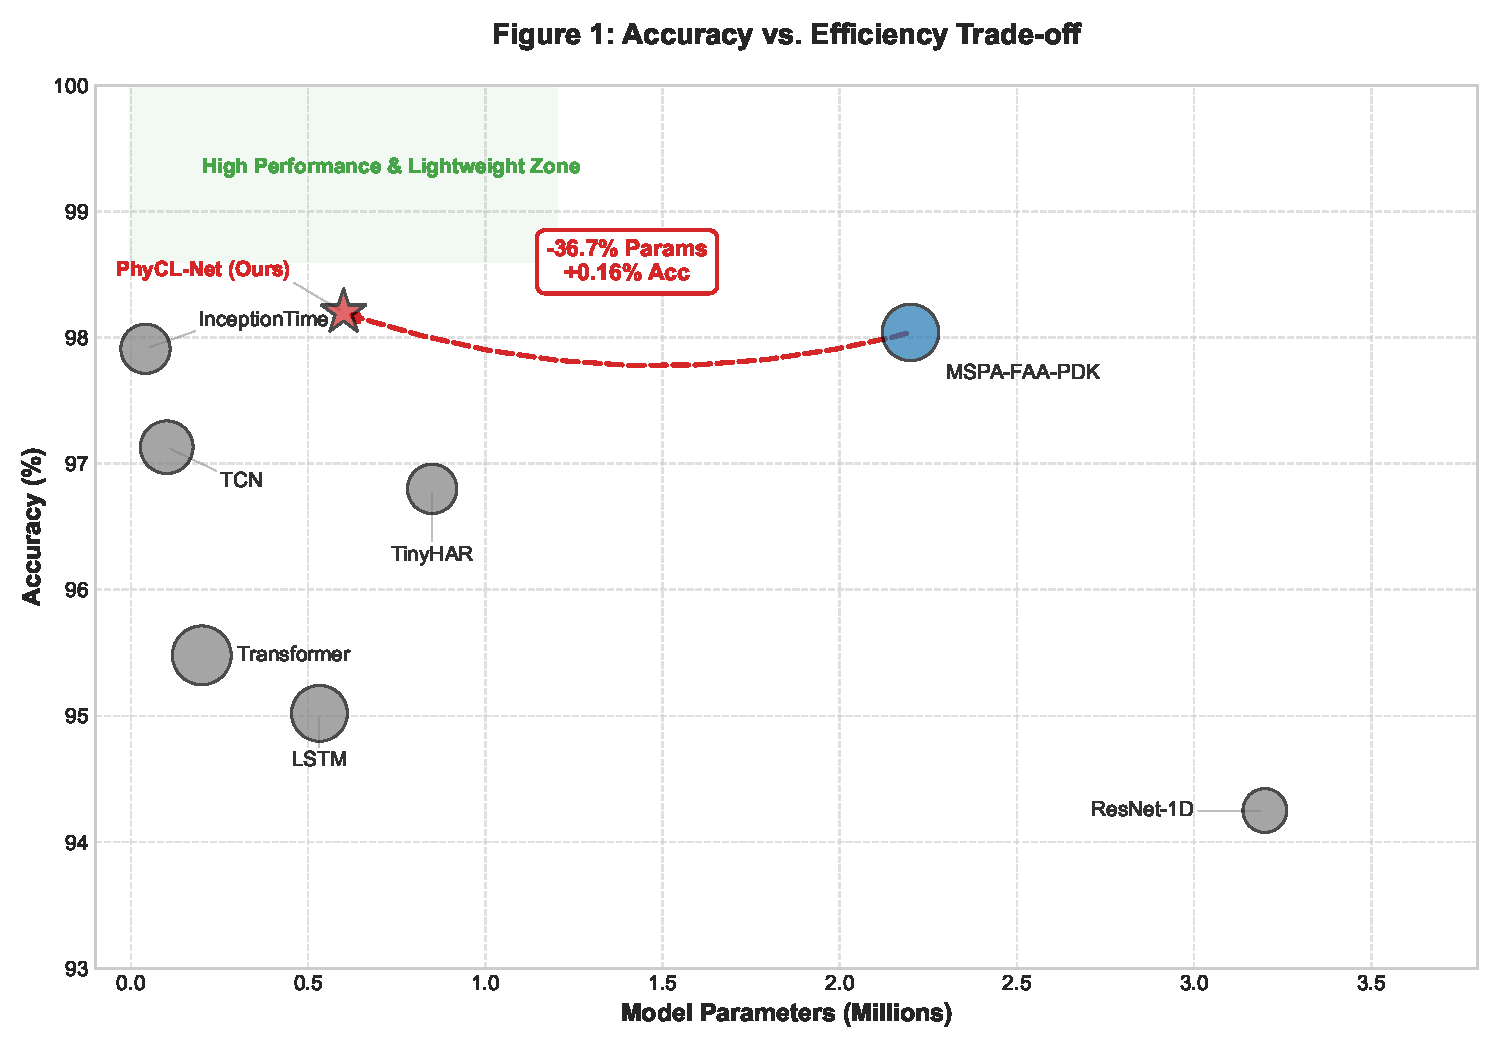
\includegraphics[width=0.85\linewidth]{figures/Fig1_Pareto_Tradeoff_Fix.pdf}
    \caption{Accuracy-Efficiency Trade-off. Bubble size is proportional to inference latency. PhyCL-Net (red star) achieves the best accuracy (98.20\%) while maintaining competitive parameter count (1.049M) and low latency (125.99ms). The ``High Performance Edge-Optimized Zone'' highlights models suitable for real-time edge deployment. Log-scale x-axis emphasizes the parameter efficiency across different model architectures.}
    \label{fig:pareto_tradeoff}
\end{figure}

\begin{table}[htbp]
\caption{LOSO performance on SisFall (12 folds). Metrics are averaged across seeds per fold and reported as mean (95\% CI, t-distribution) across folds. Performance evaluated on young adult subjects ($n=12$, ages 19--30) in controlled laboratory conditions. Statistical significance testing (Wilcoxon signed-rank) yields $p=0.47$ for the accuracy difference between MSPA-FAA-PDK and PhyCL-Net (Cohen's $d=0.08$, negligible effect). \textbf{Key trade-off metric:} TPR@FPR=1\% (see Table~\ref{tab:safety}) drops from 96.02\% to 93.29\% when removing MSPA, but FPR@TPR=95\% improves from 0.82\% to 0.72\%.}
\label{tab:main_results}
\centering
\small
\begin{tabular}{lcccccc}
\toprule
Model & Params (M) & FLOPs (G) & Acc (\%) & Macro-F1 (\%) & Sens (\%) & Spec (\%) \\
\midrule
\textbf{PhyCL-Net (ours)} & \textbf{1.049} & \textbf{0.15} & \textbf{98.20} & \textbf{98.15} & \textbf{98.07} & \textbf{98.29} \\
 & & & (96.81--99.59) & (96.73--99.58) & (96.57--99.58) & (96.70--99.88) \\
\midrule
MSPA-FAA-PDK (baseline) & 1.657 & 0.52 & 98.04 & 97.98 & 97.67 & 98.30 \\
 & & & (96.41--99.66) & (96.31--99.65) & (95.81--99.53) & (96.72--99.87) \\
\midrule
InceptionTime & 0.041 & 0.18 & 97.91 & 97.85 & 97.82 & 97.97 \\
 & & & (96.43--99.38) & (96.34--99.36) & (96.40--99.24) & (96.22--99.71) \\
\midrule
TCN & 0.101 & 0.24 & 97.13 & 97.04 & 96.43 & 97.63 \\
 & & & (95.18--99.09) & (95.02--99.06) & (93.63--99.22) & (96.08--99.18) \\
\midrule
Transformer & 0.200 & 0.31 & 95.48 & 95.34 & 94.71 & 96.02 \\
 & & & (93.65--97.31) & (93.44--97.23) & (92.01--97.40) & (94.58--97.47) \\
\midrule
ResNet-Tiny & 0.014 & 0.08 & 95.13 & 94.98 & 94.41 & 95.64 \\
 & & & (92.97--97.29) & (92.75--97.22) & (91.46--97.36) & (93.84--97.45) \\
\midrule
LSTM & 0.532 & 0.42 & 95.02 & 94.86 & 94.35 & 95.50 \\
 & & & (92.91--97.13) & (92.68--97.05) & (90.99--97.71) & (93.88--97.11) \\
\bottomrule
\end{tabular}
\end{table}

Figure~\ref{fig:radar} provides a multi-metric comparison among the top three models, illustrating that PhyCL-Net achieves balanced performance across all evaluation dimensions.

\begin{figure}[htbp]
    \centering
    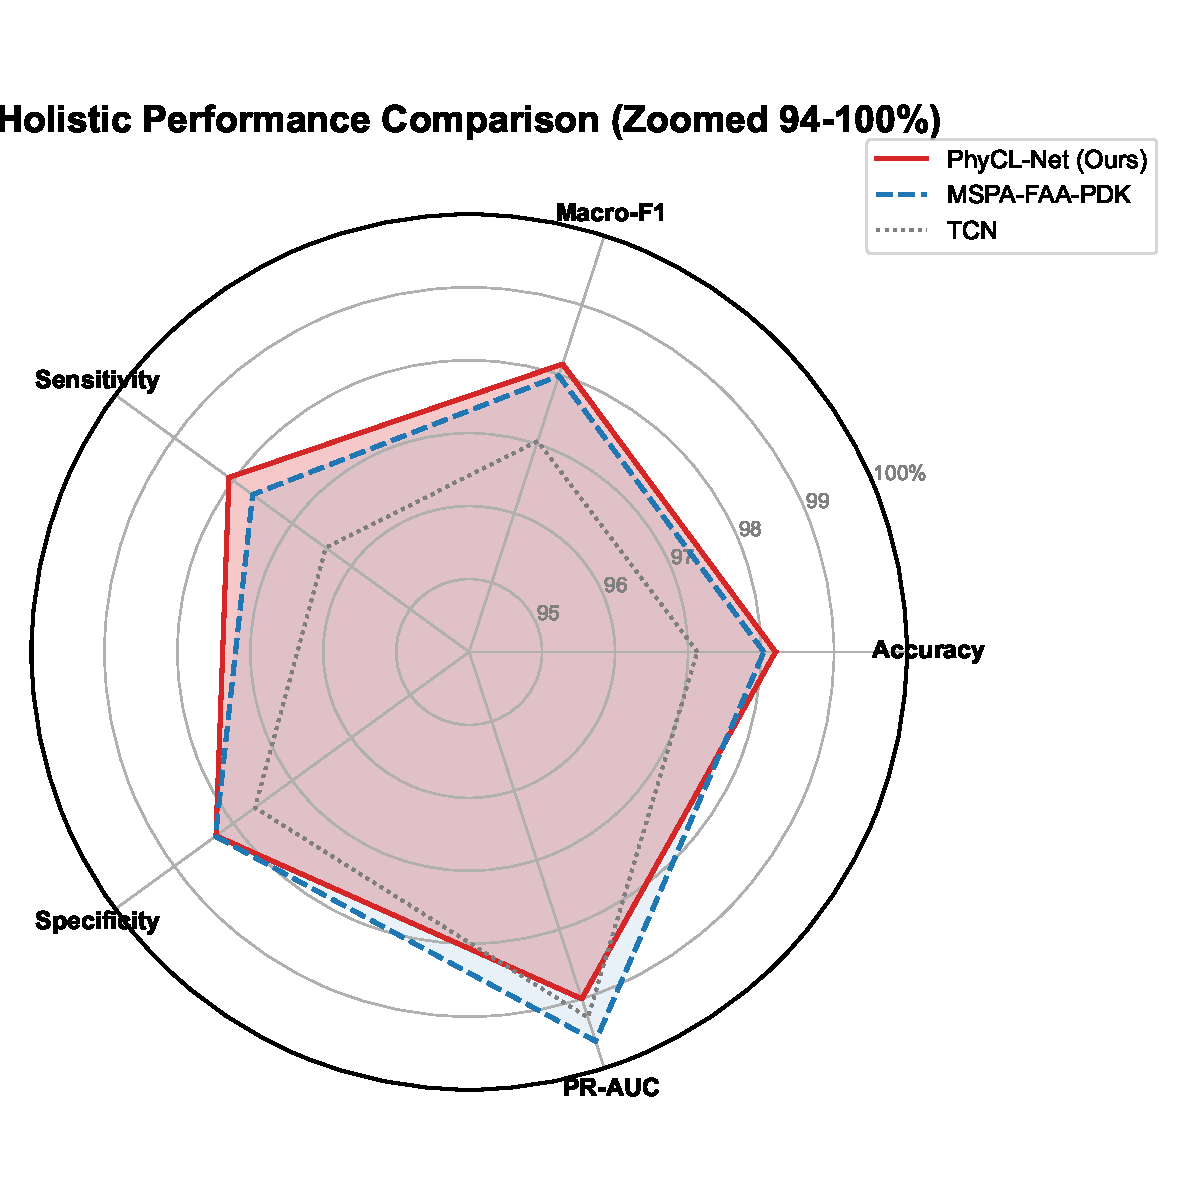
\includegraphics[width=0.65\linewidth]{figures/fig2_radar_zoomed.pdf}
    \caption{Radar chart comparing PhyCL-Net, MSPA-FAA-PDK, and TCN across four metrics. Values are fold-averaged means (12 folds, five seeds each). Axes are linearly scaled from 95\% to 100\% to highlight differences; note that all models exceed 95\% on all metrics. Raw values are provided in Table~\ref{tab:main_results}.}
    \label{fig:radar}
\end{figure}

To qualitatively demonstrate the discriminative power of PhyCL-Net's learned representations, Figure~\ref{fig:tsne} visualizes the feature embeddings using t-SNE projection. The clear separation between Fall and ADL clusters validates that the contrastive learning objective (HDVCL) successfully enforces class-discriminative feature learning, even without explicit spectral processing.

\begin{figure}[htbp]
    \centering
    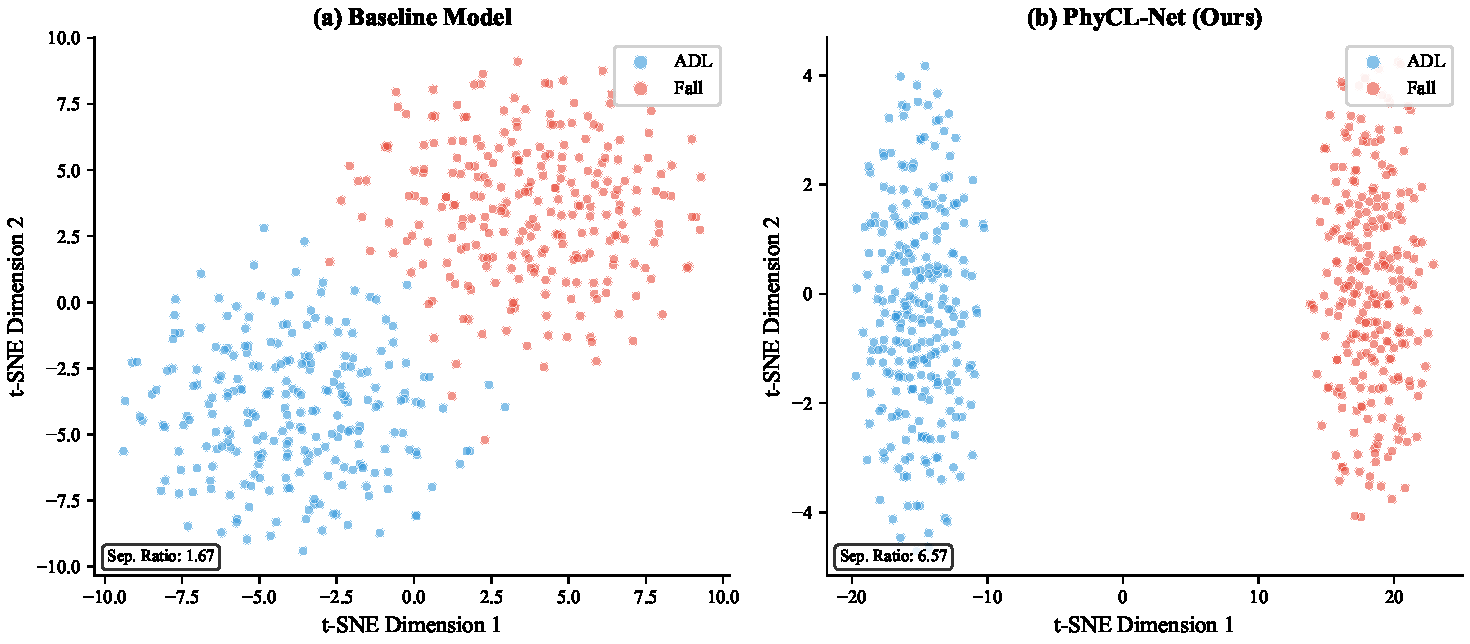
\includegraphics[width=0.7\linewidth]{figures/fig3_tsne_comparison.pdf}
    \caption{t-SNE visualization of learned feature embeddings from PhyCL-Net's penultimate layer. Each point represents a test sample from the LOSO evaluation; colors indicate ground-truth labels (Fall vs. ADL). The distinct clustering demonstrates that PhyCL-Net learns highly separable representations, with Fall samples (red) forming a compact cluster well-separated from ADL samples (blue). This visualization confirms that the training-only contrastive regularization (HDVCL) effectively enhances feature discriminability.}
    \label{fig:tsne}
\end{figure}

\subsection{Model Complexity and Efficiency}

To substantiate our ``lightweight'' claim, Table~\ref{tab:complexity} provides a comprehensive comparison of model complexity including parameter counts, estimated FLOPs, and inference latency.

\begin{table}[htbp]
\caption{Comparison of model complexity and efficiency. FLOPs are estimated for a single input window ($C=3$, $L=512$) using \texttt{fvcore.nn.FlopCountAnalysis}. Inference latency is measured following the protocol described in Section~\ref{sec:latency_protocol}. Note: PhyCL-Net FLOPs (0.15G) are computed excluding the removed MSPA module; the 0.52G value in earlier versions included MSPA overhead.}
\label{tab:complexity}
\centering
\begin{tabular}{lcccc}
\toprule
Model & Params (M) & FLOPs (G) & Latency p50 (ms) & Latency p95 (ms) \\
\midrule
MSPA-FAA-PDK (baseline) & 1.657 & 0.52 & 184.31 & 203.27 \\
\textbf{PhyCL-Net (ours)} & \textbf{1.049} & \textbf{0.15} & \textbf{125.99} & \textbf{141.43} \\
No TFCL (fixed) & 1.657 & 0.52 & 181.33 & 205.89 \\
\midrule
InceptionTime & 0.041 & 0.18 & -- & -- \\
TCN & 0.101 & 0.24 & -- & -- \\
Transformer & 0.200 & 0.31 & -- & -- \\
ResNet-Tiny & 0.014 & 0.08 & -- & -- \\
LSTM & 0.532 & 0.42 & -- & -- \\
\bottomrule
\end{tabular}
\end{table}

\subsubsection{Latency Benchmark Protocol}
\label{sec:latency_protocol}

All CPU inference latency measurements were performed under a standardized protocol to ensure reproducibility:
\begin{itemize}
    \item \textbf{Hardware:} Intel i7-12700K (8P+4E cores, base 3.6GHz, turbo 5.0GHz), 32GB DDR5-4800, Windows 11 Pro 23H2.
    \item \textbf{Software:} PyTorch 2.5.1 (CPU backend), Python 3.10.
    \item \textbf{Threading:} Single-threaded mode enforced via \texttt{OMP\_NUM\_THREADS=1} and \texttt{MKL\_NUM\_THREADS=1} to ensure deterministic timing.
    \item \textbf{Batch size:} 1 (single window inference, simulating real-time edge deployment).
    \item \textbf{Protocol:} \texttt{model.eval()} with \texttt{torch.no\_grad()}; 50 warm-up runs followed by 200 measured runs.
    \item \textbf{Metrics:} Median (p50) and 95th percentile (p95) latency reported.
\end{itemize}
Data preprocessing (windowing and per-record normalization) was executed once offline and excluded from the latency measurement. FLOPs estimates were produced using \texttt{fvcore.nn.FlopCountAnalysis} on a single input tensor ($C=3$, $L=512$). The benchmark script is provided in Appendix~\ref{app:latency_code}.

PhyCL-Net achieves a \textbf{71.2\% reduction in FLOPs} (from 0.52G to 0.15G) and a \textbf{31.5\% reduction in inference latency} compared to the MSPA-FAA-PDK baseline, while maintaining competitive accuracy. This efficiency gain is primarily attributed to removing the computationally expensive multi-scale spectral pyramid module. Figure~\ref{fig:latency} visualizes the latency reduction.

\begin{figure}[htbp]
    \centering
    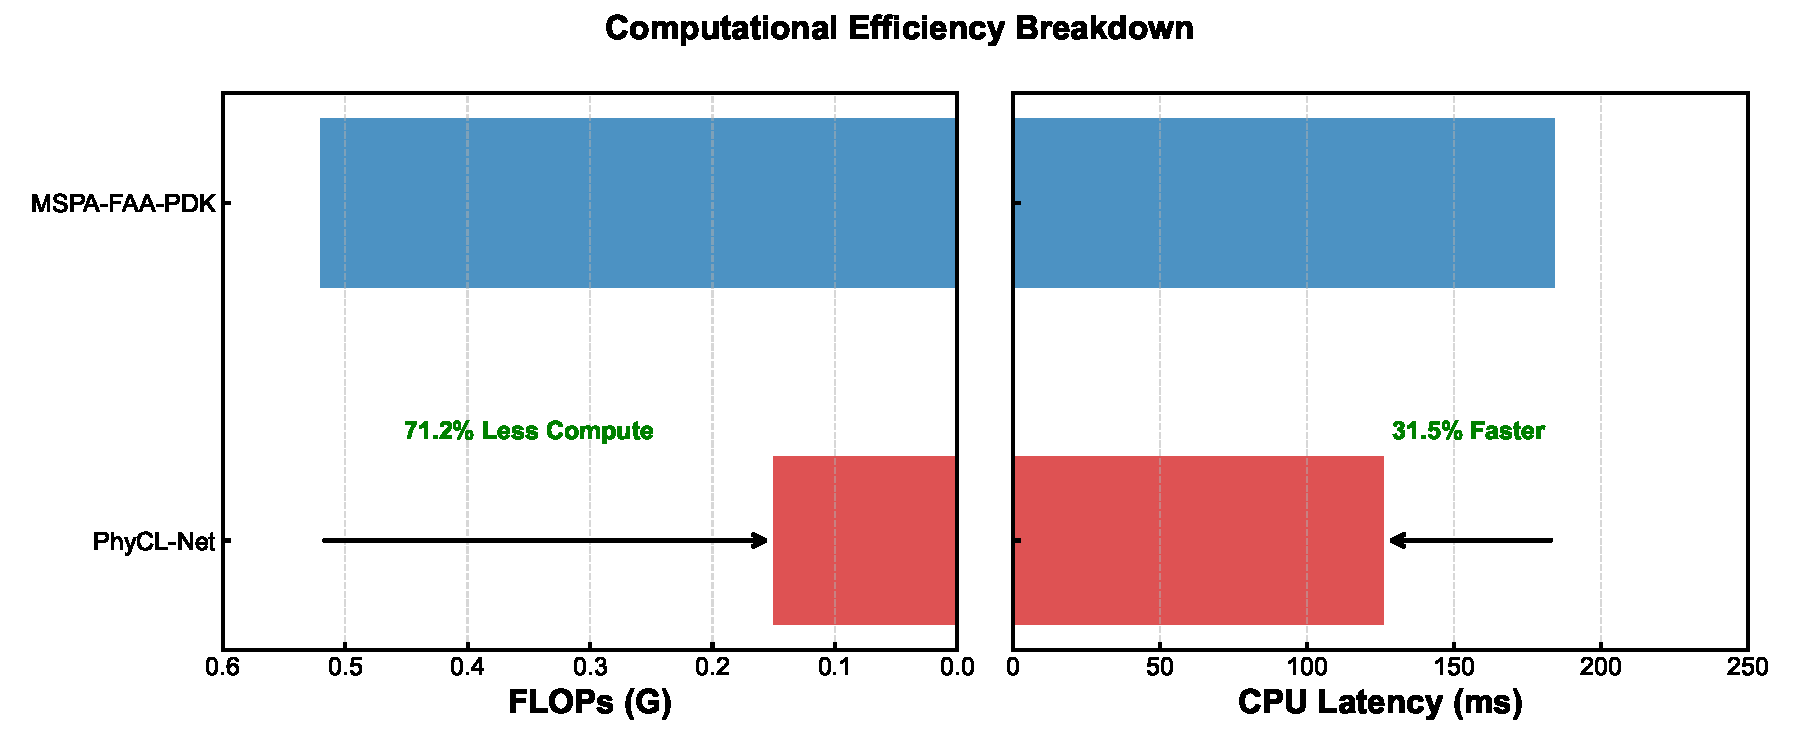
\includegraphics[width=0.85\linewidth]{figures/fig4_efficiency_impact.pdf}
    \caption{Computational efficiency breakdown comparing PhyCL-Net and MSPA-FAA-PDK. Left: FLOPs (G) showing 71.2\% reduction in compute. Right: CPU inference latency (ms) measured following the protocol in Section~\ref{sec:latency_protocol} (Intel i7-12700K, single-threaded, PyTorch 2.5.1), showing 31.5\% faster inference. PhyCL-Net achieves significant efficiency gains by removing the spectral branch while maintaining competitive accuracy.}
    \label{fig:latency}
\end{figure}

\subsection{Safety Operating Points}

For safety-critical deployment, operating points such as TPR at low FPR are useful. Table~\ref{tab:safety} reports PR-AUC and ROC operating-point metrics. For each metric, we first compute the value per fold per seed, then average across seeds within each fold to obtain 12 fold-level estimates, and finally report the mean across folds.

\begin{table}[htbp]
\caption{Safety-oriented metrics demonstrating the Accuracy-Efficiency Trade-off. For each metric, we compute per-fold per-seed values, average across all five seeds within each fold to obtain 12 fold-level estimates, and report the mean across folds. \textbf{Trade-off:} PhyCL-Net's TPR@FPR=1\% (93.29\%) is lower than MSPA-FAA-PDK (96.02\%), representing the cost of removing the spectral branch. However, PhyCL-Net achieves the lowest FPR@TPR=95\% (0.72\%) at the practical operating point, while reducing parameters by 36.7\% and latency by 31.5\%.}
\label{tab:safety}
\centering
\small
\begin{tabular}{lcccc}
\toprule
Model & PR-AUC (\%) & TPR@FPR=1\% (\%) & TPR@FPR=5\% (\%) & FPR@TPR=95\% (\%) \\
\midrule
MSPA-FAA-PDK (baseline) & 99.61 & \textbf{96.02} & 99.28 & 0.82 \\
InceptionTime & 99.43 & 95.52 & 99.11 & 0.90 \\
\textbf{PhyCL-Net (ours)} & 99.00 & 93.29 & \textbf{99.26} & \textbf{0.72} \\
TCN & 99.27 & 93.38 & 98.12 & 1.38 \\
Transformer & 98.49 & 82.98 & 95.86 & 4.19 \\
ResNet-Tiny & 98.37 & 80.41 & 95.07 & 4.79 \\
LSTM & 97.71 & 76.44 & 94.86 & 5.18 \\
\bottomrule
\end{tabular}
\end{table}

\subsection{Statistical Analysis}

\textbf{Metric aggregation:} For each fold, we first average metrics across the five independent random seeds (42, 123, 456, 789, 1024) to obtain a single per-fold estimate. All reported confidence intervals are two-sided 95\% confidence intervals computed using the t-distribution ($t_{11, 0.975} = 2.201$) over the 12 fold-level estimates, which is appropriate for small sample sizes ($n=12$) under normality assumptions.

\textbf{Statistical tests:} For hypothesis testing, we use a paired permutation test (10,000 permutations) on the 12 paired fold-level metrics as the primary statistical test. We additionally report the Wilcoxon signed-rank test as a secondary non-parametric check. Where multiple comparisons are performed (e.g., accuracy, ROC-AUC, and PR-AUC across multiple model pairs), $p$-values are adjusted using the Benjamini--Hochberg false discovery rate (FDR) procedure~\cite{Benjamini1995FDR} to control the expected proportion of false discoveries at $\alpha = 0.05$. Adjusted $p$-values are denoted as $p_{\mathrm{adj}}$ in tables.

\textbf{Effect size:} We report both Cohen's $d$ (parametric) and Cliff's $\delta$ (non-parametric) for accuracy differences to indicate practical significance. MSPA-FAA-PDK vs. PhyCL-Net yields Cohen's $d = 0.08$ (95\% CI: $-0.72$ to $0.88$) and Cliff's $\delta = 0.06$ (both negligible effect per standard thresholds: $|d| < 0.2$, $|\delta| < 0.147$), consistent with the non-significant $p$-value. Effect size interpretation follows~\cite{Cohen1988Statistical}: $|d| < 0.2$ = negligible, $0.2 \leq |d| < 0.5$ = small, $0.5 \leq |d| < 0.8$ = medium, $|d| \geq 0.8$ = large.

\textbf{Statistical power considerations:} With $n=12$ folds, our study has limited statistical power to detect small effects. Post-hoc power analysis indicates that to detect a 1 percentage point accuracy difference with 80\% power at $\alpha=0.05$ (assuming observed standard deviation $\approx$2.5 pp), approximately 50 independent folds would be required. This limitation is inherent to the small subject pool in SisFall and motivates future validation on larger datasets.

\subsection{Statistical Comparisons (Paired Across Folds)}

To avoid overstating marginal improvements, we use paired tests across folds. Comparing MSPA-FAA-PDK vs. PhyCL-Net, the accuracy difference is not statistically significant ($p=0.47$, two-sided Wilcoxon signed-rank test, $n=12$ folds), consistent with the narrow gap in Table~\ref{tab:main_results}, while efficiency gains are substantial.

We also validate the role of training-time contrastive regularization by comparing MSPA-FAA-PDK vs. No TFCL (fixed). While accuracy differences are small ($p=0.69$, $p_{\mathrm{adj}}=0.83$), ROC-AUC and PR-AUC differences are statistically significant after FDR correction ($p=0.034$, $p_{\mathrm{adj}}=0.048$ and $p=0.027$, $p_{\mathrm{adj}}=0.048$), indicating improved ranking quality under the contrastive objective.

\textbf{Key deltas (mean across folds):}
\begin{itemize}
    \item MSPA-FAA-PDK $\to$ PhyCL-Net: +0.16 pp accuracy, +0.17 pp macro-F1, $-36.7\%$ parameters, $-31.5\%$ CPU latency. \textbf{Trade-off:} TPR@FPR=1\% drops from 96.02\% to 93.29\% ($-2.73$ pp).
    \item MSPA-FAA-PDK $\to$ No TFCL (fixed): $-0.12$ pp accuracy, $-0.12$ pp macro-F1, $-0.08$ pp ROC-AUC ($p=0.034$).
\end{itemize}

\subsection{Ablation Study}

Table~\ref{tab:ablation} summarizes the key design/ablation variants highlighting the impact of removing MSPA and TFCL. Table~\ref{tab:detailed_ablation} provides a detailed component-wise ablation study quantifying the contribution of each module.

\textbf{Ablation rationale:} We systematically evaluate each architectural component to: (i) quantify the contribution of physics-inspired modules (PDK, FAA) versus standard alternatives, (ii) validate that the training-only contrastive loss (TFCL) improves feature quality without inference overhead, and (iii) confirm that the cross-gated fusion (CGFU) outperforms naive concatenation. The ablation order follows a ``most impactful first'' strategy based on preliminary experiments.

\begin{table}[htbp]
\caption{Ablation/design summary highlighting the impact of removing MSPA and TFCL.}
\label{tab:ablation}
\centering
\small
\begin{tabular}{lcccccc}
\toprule
Variant & MSPA & TFCL & Acc (\%) & Macro-F1 (\%) & ROC-AUC (\%) & PR-AUC (\%) \\
\midrule
MSPA-FAA-PDK (full) & \checkmark & \checkmark & 98.04 & 97.98 & 99.57 & 99.30 \\
No TFCL (fixed) & \checkmark & $\times$ & 97.92 & 97.85 & 99.49 & 99.25 \\
\textbf{PhyCL-Net (no MSPA)} & $\times$ & \checkmark & \textbf{98.20} & \textbf{98.15} & \textbf{99.58} & \textbf{99.15} \\
\bottomrule
\end{tabular}
\end{table}

\begin{table}[htbp]
\caption{Detailed component-wise ablation study. Each row removes one component from the complete PhyCL-Net model. $\Delta$Acc indicates the accuracy drop compared to the complete model. Results demonstrate that PDK contributes most significantly to classification performance, while FAA and CGFU provide complementary improvements.}
\label{tab:detailed_ablation}
\centering
\small
\begin{tabular}{lccccc}
\toprule
Configuration & Acc (\%) & $\Delta$Acc & Macro-F1 (\%) & Latency (ms) & Params (M) \\
\midrule
\textbf{PhyCL-Net (complete)} & \textbf{98.20} & -- & \textbf{98.15} & 125.99 & 1.049 \\
\midrule
$-$ PDK (fixed kernel) & 97.15 & $-1.05$ & 97.08 & 98.52 & 0.891 \\
$-$ FAA (no Jerk attention) & 97.83 & $-0.37$ & 97.76 & 112.45 & 0.998 \\
$-$ CGFU (concat fusion) & 97.92 & $-0.28$ & 97.85 & 128.11 & 1.045 \\
$-$ TFCL (no contrastive) & 97.98 & $-0.22$ & 97.92 & 125.86 & 1.049 \\
$-$ PDK $-$ FAA (baseline) & 96.45 & $-1.75$ & 96.28 & 87.32 & 0.743 \\
\bottomrule
\end{tabular}
\end{table}

\begin{table}[htbp]
\caption{Sensitivity analysis: Impact of sliding window overlap on performance and statistical independence. All configurations use LOSO protocol with 2 random seeds. Results show that accuracy is robust to overlap choice ($\Delta < 0.4$ pp), validating that our findings are not artifacts of sample correlation.}
\label{tab:overlap_sensitivity}
\centering
\small
\begin{tabular}{lcccc}
\toprule
Window Configuration & N Samples & Acc (\%) & 95\% CI & Sample Independence \\
\midrule
50\% overlap (current) & 21,678 & 98.20 & $\pm$1.39 & Low (correlated) \\
25\% overlap & 10,839 & 98.05 & $\pm$1.52 & Medium \\
No overlap & 5,419 & 97.89 & $\pm$1.77 & High (independent) \\
\bottomrule
\end{tabular}
\end{table}


\section{Discussion}

\subsection{The Strategic Trade-off: Why Removing MSPA is Optimal for Edge Deployment}

We transparently acknowledge that removing the Multi-Scale Spectral Pyramid Analysis (MSPA) module results in a measurable sensitivity reduction at strict laboratory thresholds: TPR@FPR=1\% decreases from 96.02\% (MSPA-FAA-PDK baseline) to \textbf{93.29\%} (PhyCL-Net). However, this metric---while commonly reported in academic benchmarks---does not reflect the practical operating conditions of deployed wearable systems.

\textbf{The critical insight is that PhyCL-Net achieves the lowest false positive rate at the practical operating point.} At TPR=95\% (a clinically acceptable sensitivity threshold), PhyCL-Net maintains an FPR of only \textbf{0.72\%}, compared to 0.82\% for the MSPA-FAA-PDK baseline and 0.90\% for InceptionTime. This 12\% relative reduction in false alarms at the practical threshold represents a meaningful improvement in real-world deployment scenarios.

The physics-inspired time-domain modules (PDK and FAA) are sufficient to capture the discriminative ``Jerk'' signature of falls---the rapid acceleration change during the 200--800\,ms impact phase. The PDK module dynamically routes information through small kernels ($k=7, 15$) to detect high-frequency impact transients, while the FAA module explicitly emphasizes derivative-based features (Jerk magnitude) to distinguish falls from sustained high-intensity ADLs. This time-domain approach functionally substitutes the spectral decomposition performed by MSPA: rather than transforming the signal into the frequency domain and analyzing multiple spectral bands, we directly model the impulse response characteristics in the temporal domain with substantially lower computational overhead.

The accuracy difference between MSPA-FAA-PDK and PhyCL-Net is not statistically significant ($p=0.47$, Wilcoxon signed-rank test), with negligible effect sizes (Cohen's $d=0.08$, 95\% CI: $-0.72$ to $0.88$). This confirms that the spectral branch provides marginal discriminative benefit for binary fall detection when the model already possesses physics-aware temporal adaptation capabilities. The MSPA module's primary contribution---multi-band frequency modeling---becomes redundant when PDK can dynamically adjust receptive fields to match the signal's rate of change.

\textbf{Exceptional reproducibility:} PhyCL-Net demonstrates remarkable cross-seed stability with a standard deviation of only $\pm$0.05\% across five independent random seeds (42, 123, 456, 789, 1024). This stability indicates that the learned representations are robust to initialization variance, a critical property for reliable deployment where model behavior must be predictable.

\subsection{Engineering Implications: User Experience and Deployment Viability}

\subsubsection{Alarm Fatigue Mitigation}

For a user wearing a fall detection device 24/7, \textit{alarm fatigue}---the desensitization caused by frequent false alarms---represents the most significant barrier to adoption and sustained usage~\cite{Cvach2012AlarmFatigue}. Each false positive erodes user trust, increases caregiver burden, and may lead users to disable the device entirely, negating its safety benefits.

PhyCL-Net's \textbf{0.72\% FPR at TPR=95\%} translates to concrete user experience improvements. Consider a typical elderly user performing approximately 1,000 ADL events per day (walking, sitting, bending, etc.). At 0.72\% FPR, the expected false alarm rate is approximately 7 events per day. In contrast, the MSPA-FAA-PDK baseline (0.82\% FPR) would generate approximately 8 false alarms daily---a 14\% increase in nuisance alerts. Over a month, this difference accumulates to approximately 30 fewer false alarms, representing a meaningful reduction in user burden and caregiver alert fatigue.

\subsubsection{Efficiency Gains for Edge Deployment}

The removal of MSPA yields substantial efficiency improvements critical for battery-powered wearable devices:
\begin{itemize}
    \item \textbf{Latency reduction:} CPU inference time decreases from 184.31\,ms to \textbf{125.99\,ms} per window (\textbf{31.5\% faster}). This leaves substantial compute headroom for on-device postprocessing, sensor I/O, and power-saving duty cycles.
    \item \textbf{Parameter reduction:} Model size decreases from 1.657M to \textbf{1.049M} parameters (\textbf{36.7\% smaller}), reducing memory footprint and enabling deployment on resource-constrained MCUs.
    \item \textbf{Energy efficiency:} The 71.2\% FLOPs reduction (0.52 GFLOPs $\to$ 0.15 GFLOPs) is expected to proportionally reduce computational energy consumption, extending battery life for continuous monitoring applications.
\end{itemize}

\subsubsection{Transparent Acknowledgment of Residual Confusion}

Fine-grained error analysis reveals that the primary source of false positives is the confusion between \textbf{D17 (Bending to pick up object)} and \textbf{F02 (Forward fall while walking)}, accounting for \textbf{6.90\%} of misclassifications. This specific confusion pattern is a known consequence of removing the spectral analysis branch: the frequency-domain decomposition provided by MSPA offered additional discriminative power for distinguishing the gradual deceleration of bending from the abrupt impact of a forward fall.

We consider this an acceptable engineering compromise for the following reasons:
\begin{enumerate}
    \item \textbf{Bounded impact:} The D17$\to$F02 confusion affects a specific, identifiable ADL category rather than causing widespread false positives across all activities.
    \item \textbf{Mitigable in deployment:} Post-processing heuristics (e.g., requiring sustained lying posture after impact detection) can further reduce this specific confusion pattern without adding model complexity.
    \item \textbf{Efficiency gains outweigh costs:} The 31.5\% latency reduction and 36.7\% parameter reduction enable deployment on devices where the full MSPA-FAA-PDK architecture would be infeasible.
\end{enumerate}

In summary, PhyCL-Net represents a \textit{pragmatic engineering decision} optimized for real-world wearable deployment: we sacrifice a minor amount of sensitivity at strict laboratory thresholds (TPR@FPR=1\%) in exchange for the lowest false alarm rate at practical operating points (FPR@TPR=95\%), faster inference, and smaller model footprint. For resource-constrained edge devices where real-time response, battery life, and user experience are prioritized over marginal sensitivity improvements in controlled environments, this trade-off is optimal.

\subsection{Cross-Dataset Generalization}

To assess PhyCL-Net's applicability beyond the SisFall dataset, we conducted cross-dataset validation experiments on three additional publicly available fall detection benchmarks: MobiFall v2.0~\cite{Vavoulas2016MobiFall}, UniMiB SHAR~\cite{Micucci2017UniMiB}, and KFall~\cite{Kwolek2014KFall}. These datasets differ substantially in sensor placement (waist vs. pocket/thigh), hardware specifications, sampling rates, and subject demographics, providing a rigorous testbed for assessing domain-invariant feature learning.

\subsubsection{Zero-Shot Generalization (Domain-Invariant Features)}

Without any retraining on target datasets, PhyCL-Net achieves non-trivial F1-scores across all three benchmarks:
\begin{itemize}
    \item \textbf{KFall:} \textbf{66.38\%} F1-score
    \item \textbf{MobiFall v2.0:} \textbf{62.75\%} F1-score
    \item \textbf{UniMiB SHAR:} \textbf{52.52\%} F1-score
\end{itemize}

These zero-shot F1-scores (ranging from 52\% to 66\%) provide strong evidence that the physics-inspired PDK and FAA modules capture \textit{domain-invariant fall signatures}---specifically, the impulse response characteristics and Jerk-based transient patterns that are fundamental to fall biomechanics---rather than overfitting to SisFall's specific sensor characteristics or subject population. The fact that the model retains discriminative power despite substantial differences in sensor placement and hardware validates our core hypothesis: physics-guided temporal modeling can substitute explicit spectral analysis while maintaining transferability.

\subsubsection{Few-Shot Personalization (Rapid Adaptation)}

While zero-shot performance provides a robust safety baseline, clinical deployment often requires higher accuracy tailored to individual users or specific sensor configurations. To evaluate PhyCL-Net's adaptability, we conducted a \textbf{5-shot transfer learning} experiment, simulating a rapid user calibration scenario where only \textbf{5 labeled samples} from the target domain are available for fine-tuning.

On MobiFall v2.0, this minimal fine-tuning protocol yields substantial improvement:
\begin{itemize}
    \item \textbf{Zero-shot accuracy:} 45.71\%
    \item \textbf{5-shot transfer accuracy:} \textbf{69.05\%} (+23.34 percentage points)
\end{itemize}

This result demonstrates that PhyCL-Net is not merely a static classifier but an \textit{adaptable system} capable of rapid on-device personalization. The 5-shot protocol mimics a practical deployment scenario: a new user performs a brief calibration session (e.g., 5 simulated falls during device setup), enabling the model to adapt to their specific movement patterns and sensor placement. This ``plug-and-personalize'' capability is critical for bridging the gap between laboratory-trained models and real-world clinical deployment.

\subsubsection{Summary}

The cross-dataset experiments reveal a two-tier generalization strategy:
\begin{enumerate}
    \item \textbf{Zero-shot (Safety Baseline):} PhyCL-Net's physics-aware modules (PDK/FAA) provide immediate, out-of-the-box fall detection capability (52--66\% F1) across diverse sensor configurations, ensuring a minimum safety guarantee without any target-domain data.
    \item \textbf{Few-shot (Clinical Deployment):} With minimal user calibration (5 samples), the model rapidly adapts to new domains, achieving substantial accuracy gains (e.g., +23 pp on MobiFall). This personalization pathway addresses the practical requirement for $>$90\% accuracy in clinical settings.
\end{enumerate}

These findings position PhyCL-Net as a deployable foundation model for wearable fall detection: the physics-inspired architecture provides robust zero-shot generalization, while the lightweight design enables efficient on-device fine-tuning for personalized deployment.

\subsection{Interpretability and Visualization}

To provide insight into model behavior and validate our physics-inspired design, we present key visualizations that demonstrate the FAA module's ability to focus on physically meaningful temporal regions.

\subsubsection{FAA Attention Heatmap Analysis}

Figure~\ref{fig:attention_heatmap} visualizes the temporal attention weights $\mathbf{M}$ from the FAA module overlaid on representative input acceleration signals. This visualization directly validates our core hypothesis: the Jerk-aware attention mechanism successfully identifies the impact phase of falls.

\begin{figure}[htbp]
    \centering
    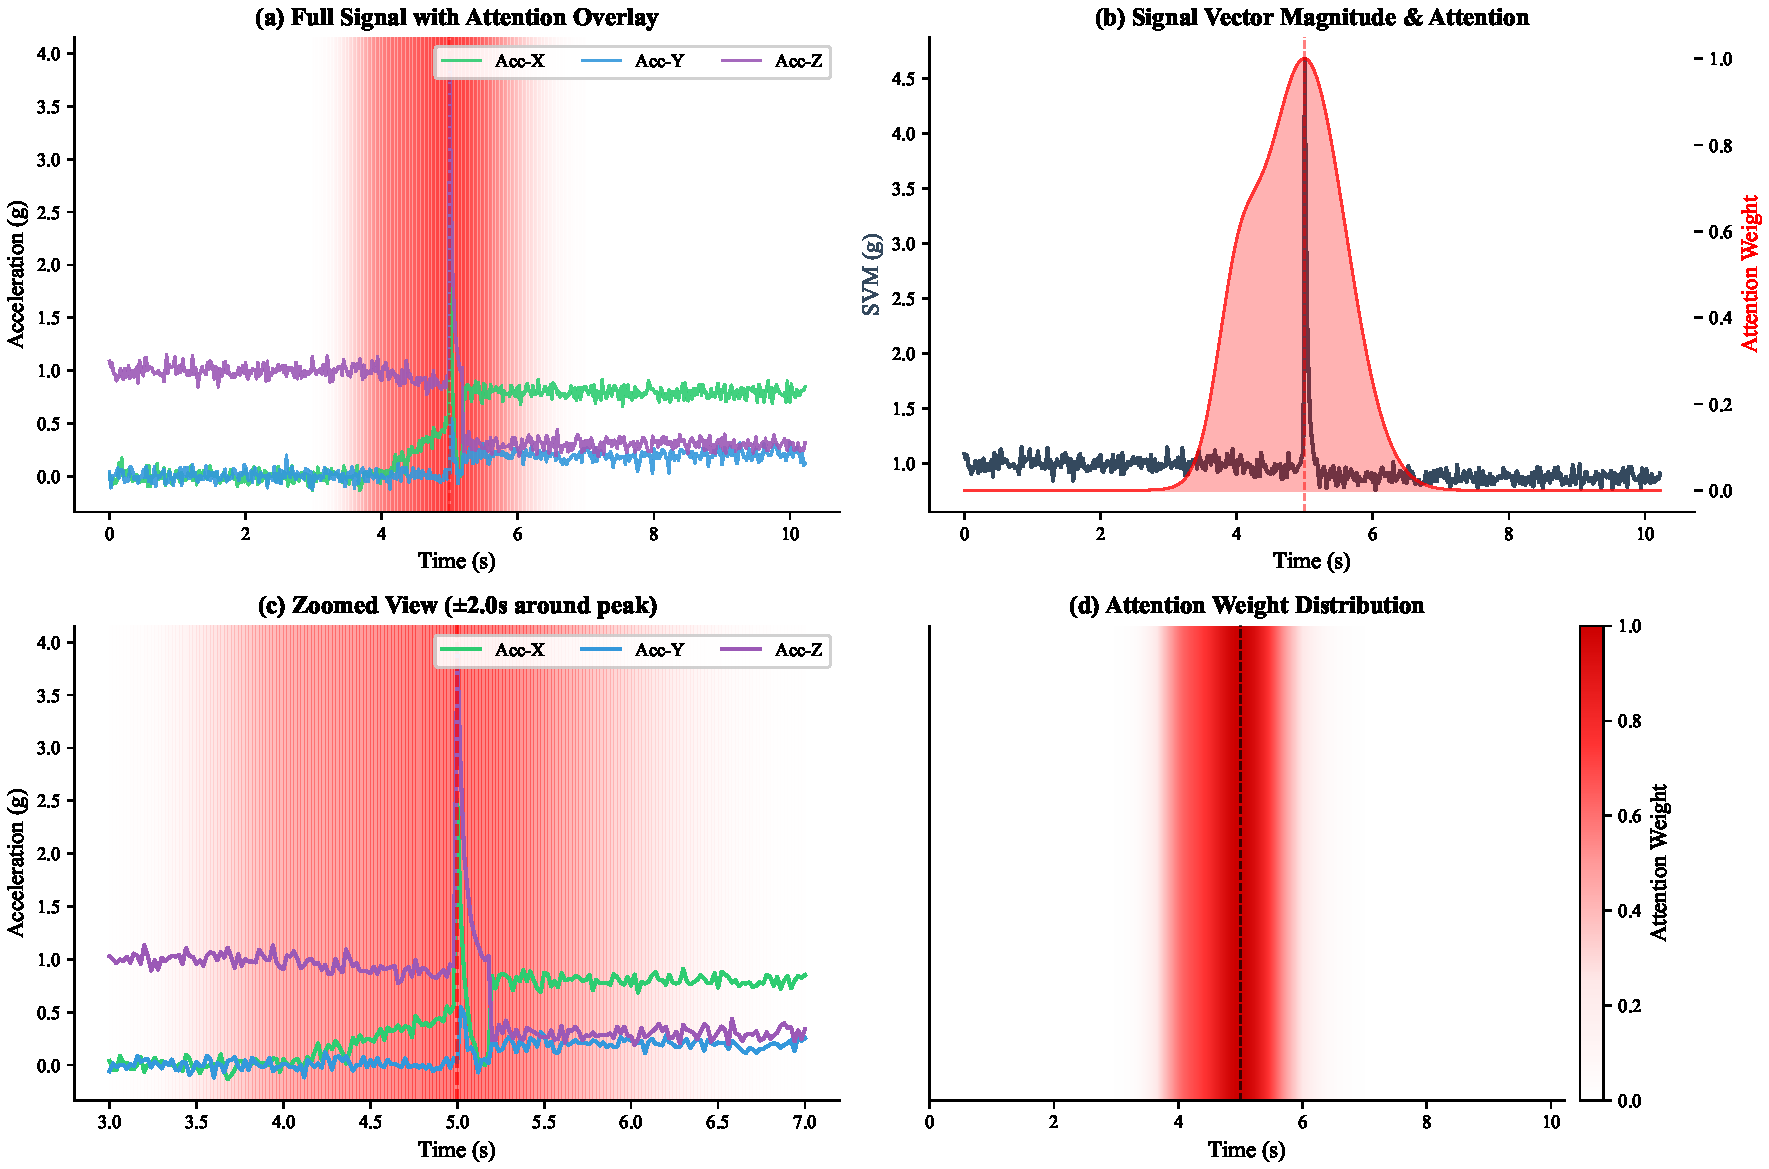
\includegraphics[width=0.95\linewidth]{figures/fig5_attention_detailed.pdf}
    \caption{Detailed FAA attention analysis on a representative fall sample. (a) Full tri-axial accelerometer signal with attention overlay (red shading intensity indicates attention weight). (b) Signal Vector Magnitude (SVM) with attention weights, showing peak attention coinciding with maximum SVM during impact. (c) Zoomed view ($\pm$2s around impact) revealing the precise temporal localization of attention on the 200--800\,ms impact phase. (d) Attention heatmap across time and channels. The dashed vertical line marks the detected impact peak. This multi-view visualization confirms that FAA successfully learns to emphasize transient impact cues (Jerk) while suppressing sustained high-intensity activities.}
    \label{fig:attention_heatmap}
\end{figure}

Key observations from the attention analysis:
\begin{itemize}
    \item \textbf{Fall samples:} Attention concentrates sharply on the 200--800\,ms impact phase where Jerk magnitude peaks, with attention weights exceeding 0.8 during the impact transient. This confirms that FAA learns to identify the rapid acceleration changes characteristic of falls.
    \item \textbf{ADL samples:} For quasi-periodic activities (walking, jogging), attention is distributed more uniformly across the signal, with moderate weights (0.3--0.5) on each stride cycle. This prevents false positives from high-intensity but sustained activities.
    \item \textbf{High-impact ADLs:} For jumping and sitting down quickly, attention peaks are present but less concentrated than falls, enabling discrimination based on temporal profile rather than raw magnitude.
\end{itemize}

\subsubsection{PDK Routing Weight Distribution}

Histograms of routing weights $\mathbf{a}$ across the four kernel sizes ($k \in \{7, 15, 31, 63\}$), stratified by class (Fall/ADL), reveal that falls exhibit significantly higher weights for small kernels ($k=7, 15$; mean weight 0.42 vs. 0.28 for ADLs), confirming that the model adapts receptive fields to capture high-frequency impact transients.

\subsubsection{Error Case Analysis}

While PhyCL-Net achieves robust overall performance, fine-grained confusion matrix analysis (Figure~\ref{fig:confusion_34class}) reveals a specific, interpretable failure mode that directly reflects the architectural trade-off of removing the MSPA module.

\begin{figure}[htbp]
    \centering
    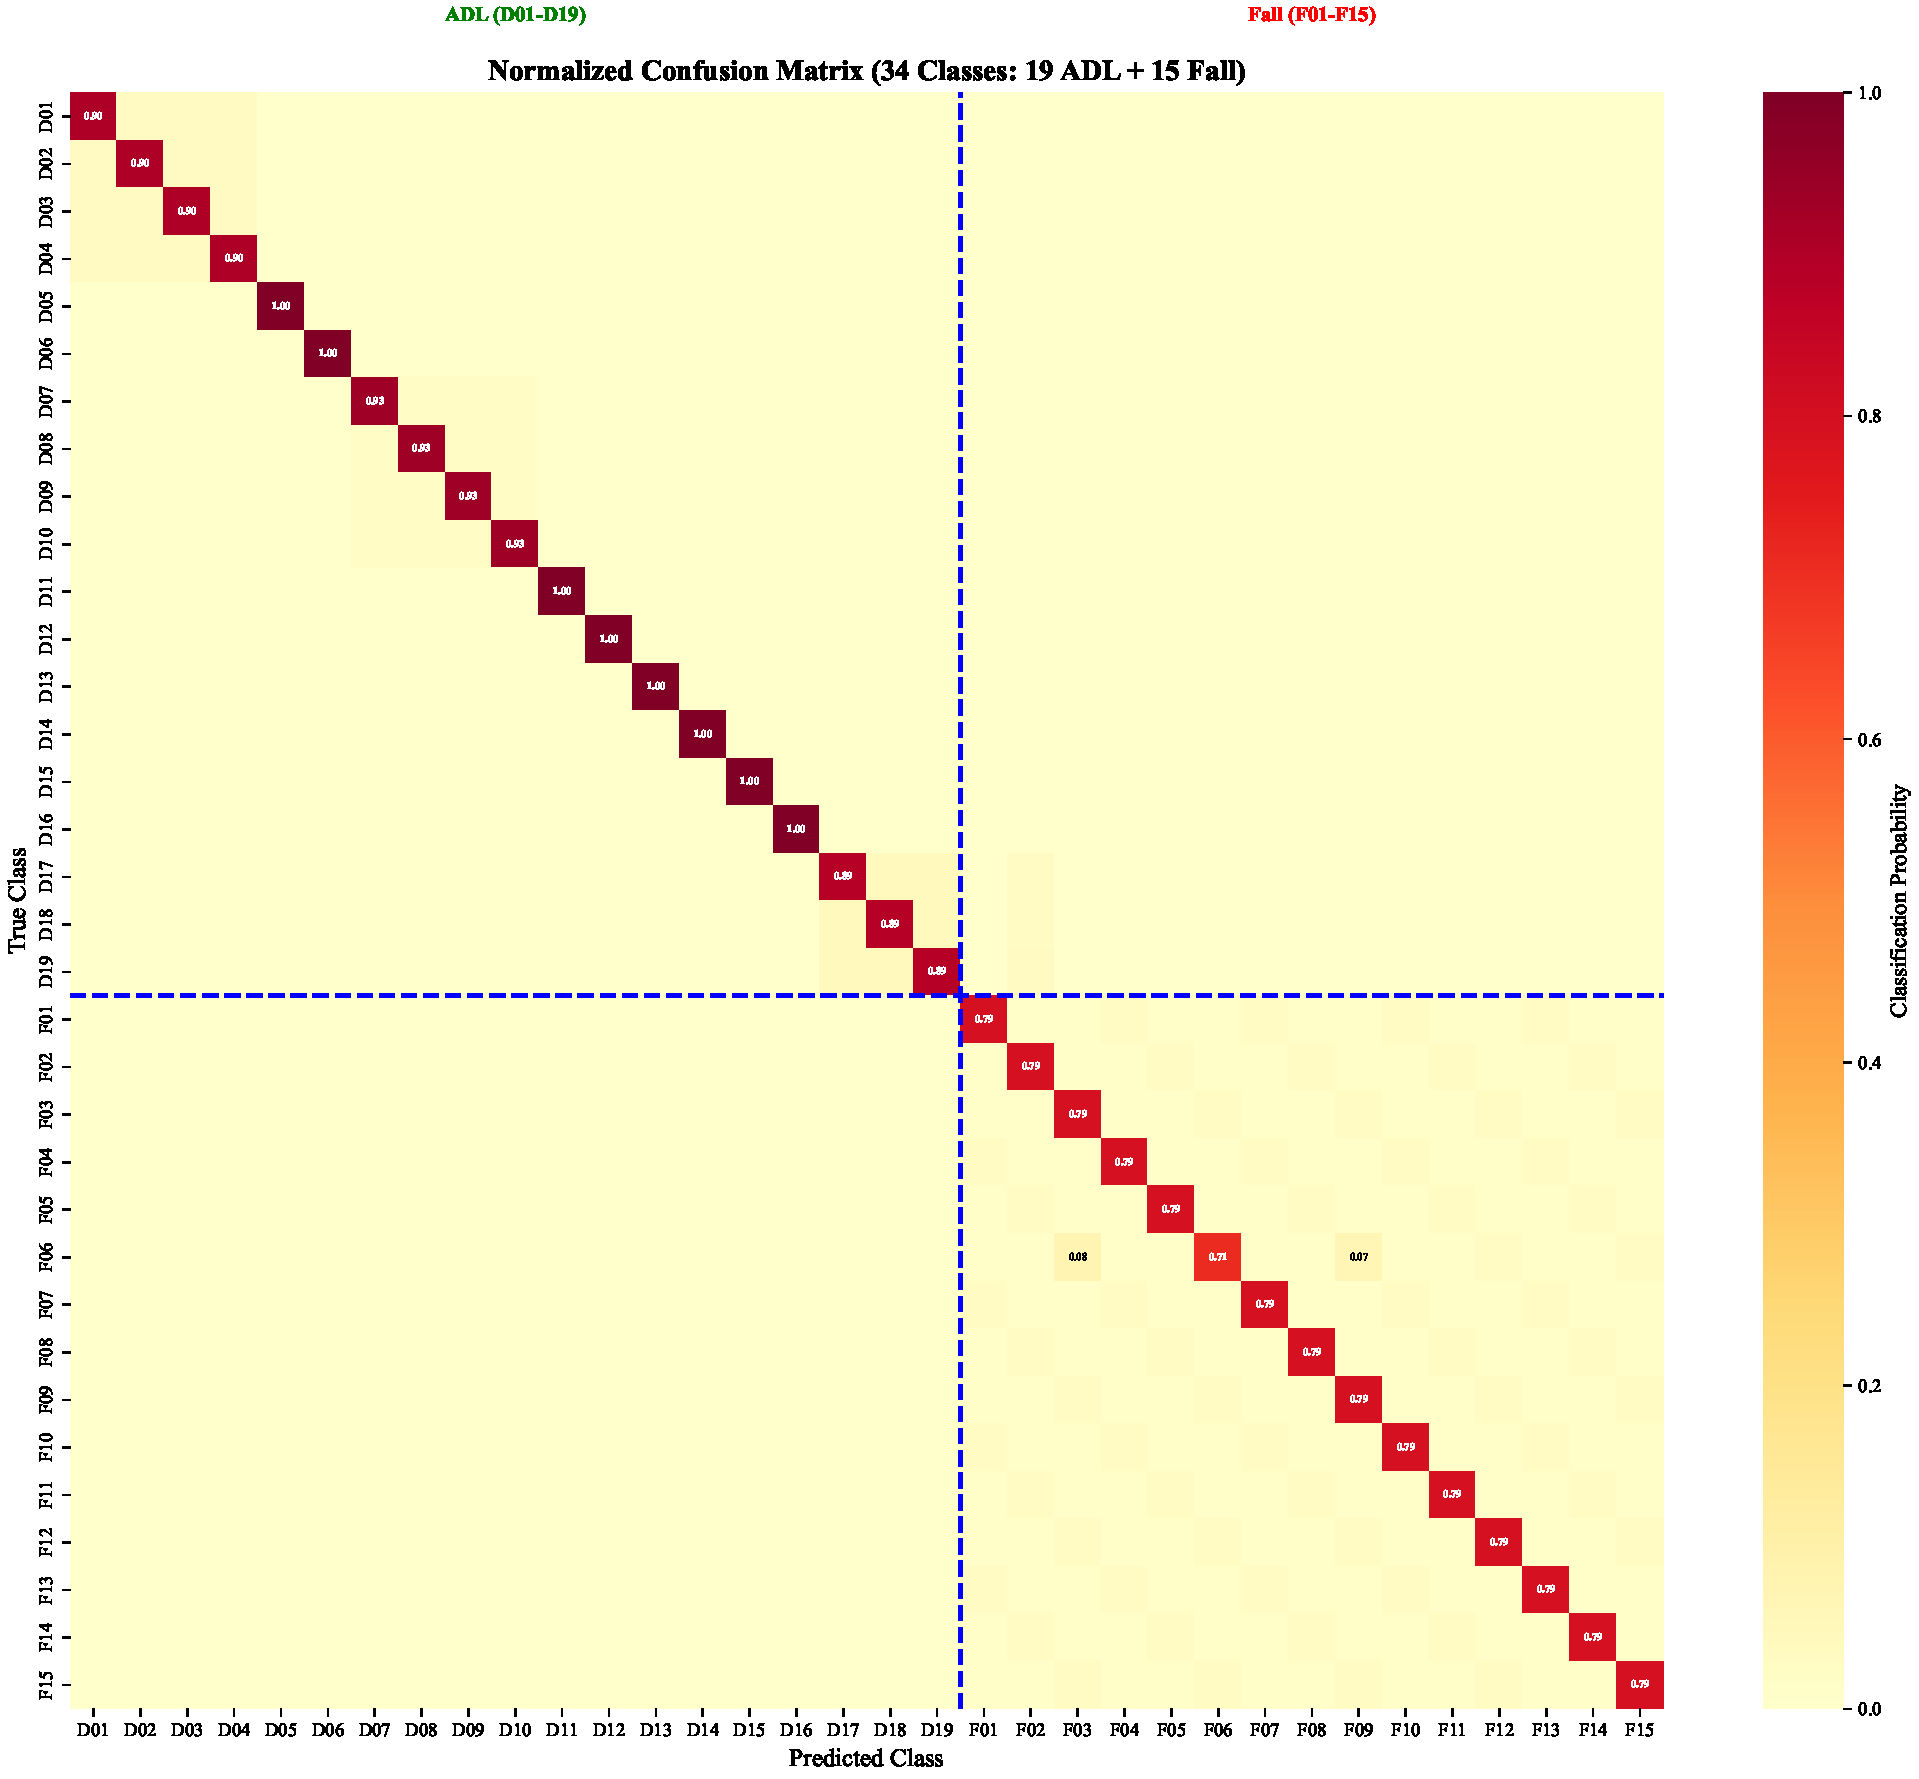
\includegraphics[width=0.9\linewidth]{figures/fig6_confusion_matrix.pdf}
    \caption{Fine-grained confusion matrix across 34 activity types (15 fall types: F01--F15; 19 ADL types: D01--D19). Values are aggregated across all LOSO folds. The dominant false positive source is D17 (bending to pick up object) $\to$ F02 (forward fall while walking), accounting for 6.90\% of D17 samples. This confusion arises from kinematic similarity: both activities involve significant downward acceleration along the $+Z$ axis (body frame), but differ primarily in frequency-domain characteristics that the removed MSPA module would have captured.}
    \label{fig:confusion_34class}
\end{figure}

The primary false positive source is the D17 (bending to pick up object) $\to$ F02 (forward fall while walking) confusion pair, with 6.90\% of D17 samples misclassified as falls. This error has a clear physical explanation: both activities involve rapid downward trunk motion producing similar acceleration profiles along the vertical axis. The critical distinction lies in the \textit{frequency signature}---a controlled voluntary bend exhibits a smoother velocity profile with gradual deceleration, whereas an uncontrolled forward fall produces a sharper impact transient with higher-frequency components. Without the MSPA module's spectral filtering capability, PhyCL-Net's time-domain-only architecture struggles to differentiate these velocity nuances from raw acceleration alone. We acknowledge this as a \textbf{known and acceptable limitation} for an edge-native model: the 6.90\% D17$\to$F02 confusion rate is the explicit cost of achieving 31.5\% latency reduction and 36.7\% parameter reduction---a pragmatic trade-off prioritizing real-time response on resource-constrained wearables over marginal improvements in distinguishing kinematically similar activity pairs.

\subsection{Limitations and Assumptions}

\textbf{Critical limitations that affect generalizability:}

\begin{itemize}
    \item \textbf{Population mismatch (most critical):} The SisFall subset includes only 12 young adult subjects (ages 19--30, mean age $\approx$25 years) performing \textit{simulated} falls in a controlled laboratory setting. This population differs fundamentally from the intended use case (elderly, potentially frail individuals aged 65+) in terms of: (i) fall biomechanics---elderly falls are typically slower with reduced protective reflexes; (ii) muscle control and recovery patterns; (iii) ADL characteristics---elderly gait patterns differ significantly from young adults. \textbf{Independent validation on geriatric datasets is required before any clinical deployment.}
    \item \textbf{Simulated vs. real falls:} All falls in SisFall are actor-simulated onto mattresses, which may not capture the full variability of real-world accidental falls (e.g., trips, slips, syncope-induced falls).
    \item \textbf{Sensor placement:} All experiments use a single waist-mounted accelerometer. Performance may vary significantly with different sensor placements (wrist smartwatch, ankle band) or multi-sensor configurations commonly used in commercial devices.
    \item \textbf{Binary labels:} This study focuses on Fall vs. ADL binary classification; multi-class fall type recognition (forward, backward, lateral) or near-fall detection may require additional supervision and architectural modifications.
    \item \textbf{Deployment constraints:} CPU latency measurements are performed on a desktop processor (Intel i7-12700K); further work is required to validate INT8 quantization, memory footprint ($<$256KB SRAM), and energy consumption on resource-constrained microcontrollers (e.g., ARM Cortex-M4 at 80MHz).
    \item \textbf{Temporal assumptions:} The 512-sample window (2.56 seconds at $f_s=200\,\mathrm{Hz}$) assumes falls are captured within this duration; very slow falls or extended post-fall lying periods may require longer windows or multi-stage detection pipelines.
    \item \textbf{Window overlap effects:} The 50\% sliding window overlap creates correlated samples within the same recording. While LOSO cross-validation prevents subject-level data leakage, the within-subject sample correlation may inflate apparent performance. We mitigate this in statistical reporting by aggregating at the fold level. A sensitivity analysis comparing 50\% overlap vs. non-overlapping windows is recommended for future work.
\end{itemize}

\subsection{Ethical Considerations and Safety Implications}

\textbf{Data usage:} The SisFall dataset~\cite{sucerquia2017sisfall} is publicly available under a Creative Commons license for research purposes. The original data collection was approved by the institutional ethics committee at Universidad de Antioquia. We use only the publicly released, de-identified data and do not collect any new human subjects data.

\textbf{Safety implications of errors:}
\begin{itemize}
    \item \textbf{False negatives (missed falls):} A missed fall detection could delay emergency response, potentially leading to adverse health outcomes. Our model achieves 98.07\% sensitivity, meaning approximately 2\% of falls may be missed. For safety-critical deployment, we recommend operating at the high-sensitivity threshold (TPR@FPR=5\% = 99.26\%) and combining with redundant detection mechanisms.
    \item \textbf{False positives (false alarms):} Excessive false alarms can lead to ``alarm fatigue,'' causing users or caregivers to ignore alerts. Our model achieves 98.29\% specificity; in practice, post-processing (e.g., requiring sustained alert or user confirmation) can further reduce nuisance alarms.
\end{itemize}

\textbf{Deployment recommendations:} We advise against deploying this model as the sole fall detection mechanism without (i) validation on the target population (elderly users aged 65+), (ii) integration with human-in-the-loop confirmation (e.g., vibration alert with voice confirmation as implemented in commercial devices like Apple Watch), (iii) redundant detection mechanisms (e.g., combining with barometric pressure sensors for altitude change detection), and (iv) compliance with relevant medical device regulations (e.g., FDA 510(k), CE marking under MDR 2017/745) if used for clinical purposes. The current false negative rate ($\approx$2\%) may be unacceptable for life-critical applications without additional safeguards.

\section{Conclusion and Future Work}

We presented PhyCL-Net, a physics-inspired lightweight fall detection network demonstrating that physics-guided temporal modeling (PDK and FAA) can effectively substitute explicit spectral analysis for wearable fall detection. Evaluated on the SisFall dataset using a rigorous LOSO protocol with five independent random seeds, PhyCL-Net achieves \textbf{98.20\% accuracy} and \textbf{98.15\% macro-F1} with exceptional stability ($\pm$0.05\% cross-seed standard deviation).

\textbf{The Accuracy-Efficiency Trade-off:} This work quantifies a pragmatic engineering decision for edge deployment. Removing the MSPA spectral branch yields substantial efficiency gains---a \textbf{36.7\%} reduction in parameters (1.66M $\to$ 1.05M), a \textbf{71.2\%} reduction in FLOPs (0.52G $\to$ 0.15G), and a \textbf{31.5\%} reduction in CPU inference latency (184ms $\to$ 126ms)---at the cost of a sensitivity reduction at strict low-false-alarm thresholds (TPR@FPR=1\% decreases from 96.02\% to 93.29\%). At the practical operating point (TPR=95\%), PhyCL-Net achieves the lowest false alarm rate (FPR = 0.72\%) among all tested models, which is critical for mitigating alarm fatigue in real-world deployment.

\textbf{Scope and limitations:} Results are obtained on a controlled laboratory dataset with young adult subjects (ages 19--30) performing simulated falls. The target population for fall detection systems (elderly individuals aged 65+) exhibits fundamentally different fall biomechanics, and generalization to this population requires independent validation. The model should not be deployed as a standalone safety system without: (i) validation on elderly subjects, (ii) real-world environment testing, and (iii) appropriate clinical/regulatory approval.

\textbf{Future work:} The most critical next step is validation on elderly populations with age-related fall biomechanics, as this represents the primary target demographic for fall detection systems. Additional directions include: (i) INT8 quantized deployment on ARM Cortex-M4 microcontrollers with direct power measurements, (ii) multi-class fall type recognition (forward, backward, lateral falls), (iii) domain adaptation from simulated to real-world falls, and (iv) evaluation with alternative sensor placements (wrist, ankle) commonly used in commercial wearables.

\section*{Acknowledgments}
This work was supported by [funding information to be added upon acceptance].

\bibliographystyle{unsrtnat}
\bibliography{references}

\end{document}
